\documentclass[aspectratio=169]{beamer}

% Theme and color scheme
\usetheme{Madrid}
\usecolortheme{seahorse}

% Packages
\usepackage[utf8]{inputenc}
\usepackage{graphicx}
\usepackage{amsmath}
\usepackage{amssymb}
\usepackage{tikz}
\usepackage{booktabs}
\usepackage{subcaption}
\usepackage{xcolor}

% Custom colors
\definecolor{rayblue}{RGB}{0, 122, 204}
\definecolor{awsorange}{RGB}{255, 153, 0}
\definecolor{hpcgreen}{RGB}{0, 153, 76}

% Title information
\title[Optimizing Vector Algorithm Processing]{Optimizing Vector Algorithm Processing through the integration of Ray IO and HPC in the Cloud}
\author{Tiago de Souza de Oliveira}
\institute[University]{
    Master's Thesis Defense \\
    Computer Science Department
}
\date{\today}

% Footer information
\setbeamertemplate{footline}[frame number]

\begin{document}

% Title slide
\frame{\titlepage}

% Slide 1: The New Frontier
\begin{frame}{The New Frontier: Scaling Scientific Workflow with ETL and AI Workloads}
    \begin{columns}
        \begin{column}{0.6\textwidth}
            \textbf{Context \& Motivation:}
            \begin{itemize}
                \item \textbf{Scientific domains} (genomics, CFD) and \textbf{Large-scale AI} (NLP, CV) rely on processing \textbf{huge datasets}
                \item Transform raw knowledge into \textcolor{rayblue}{\textbf{dense numeric arrays (embeddings)}} for downstream algorithms
                \item \textbf{HPC limitations on pre-processing:} struggles with data transformation and intensive I/O
                \item Map-Reduce/Apache Spark often \textbf{falls short at PB-scale processing and lack distributed engine for training AI models}
            \end{itemize}
        \end{column}
        \begin{column}{0.4\textwidth}
            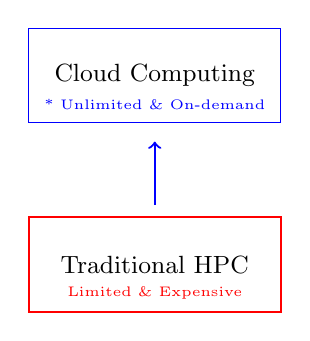
\begin{tikzpicture}[scale=0.8]
                % Traditional HPC box
                \draw[thick, red] (0,0) rectangle (4,1.5);
                \node at (2,0.75) {\small Traditional HPC};
                \node[red] at (2,0.3) {\tiny Limited \& Expensive};
                
                % Arrow
                \draw[->, thick, blue] (2, 1.7) -- (2, 2.7);
                
                % Cloud box
                \draw[blue] (0,3) rectangle (4,4.5);
                \node at (2,3.75) {\small Cloud Computing};
                \node[blue] at (2,3.3)  {\tiny * Unlimited \& On-demand};
            \end{tikzpicture}
        \end{column}
    \end{columns}
    
    \vspace{0.3cm}
    \begin{block}{The Opportunity}
        Cloud computing offers \textbf{unlimited, on-demand capacity} with better cost efficiency balance leveraging the best for IaC, Devops and Data Interoperability
    \end{block}
\end{frame}


% Slide 2: Scientific workflow
\begin{frame}{Scientific workflow}
    \begin{columns}
        \begin{column}{0.5\textwidth}
            \begin{itemize}
                \item Regular workload
                \item Embeddings to capture aditional features and integrates with numeric simulation
                \item Generative AI for enhancing input dataset
                \item Data centric to ease workloads interoperability amongs different engine processing
            \end{itemize}
        \end{column}
        \begin{column}{0.5\textwidth}
            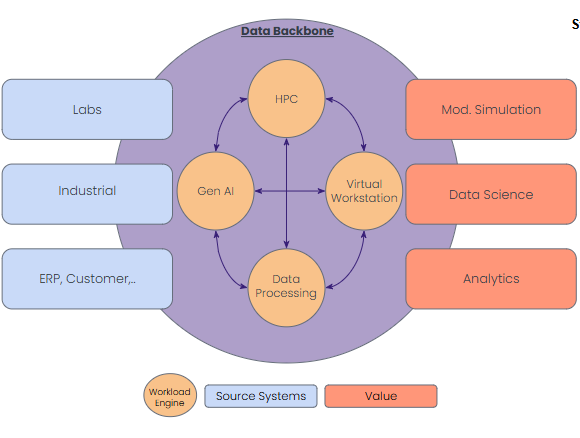
\includegraphics[width=\textwidth,height=0.6\textheight,keepaspectratio]{DataCentric-DataBackbone-Strategy.png}
        \end{column}
    \end{columns}
    
    \vspace{0.3cm}
    \begin{block}{Key Insight}
        \textbf{How embeddings can} ... for numeric simulation
    \end{block}
\end{frame}

% Slide 3: A Two-Phased
\begin{frame}{A Two-Phased Cloud-Native Architecture for Optimization}
    % Upper row with bullet points
    \begin{itemize}
        \item First bullet point about the two-phased architecture
        \item Second bullet point about cloud-native optimization
        \item Third bullet point about the integration approach
    \end{itemize}
    
    \vspace{0.4cm}
    
    % Bottom row with image
    \begin{center}
        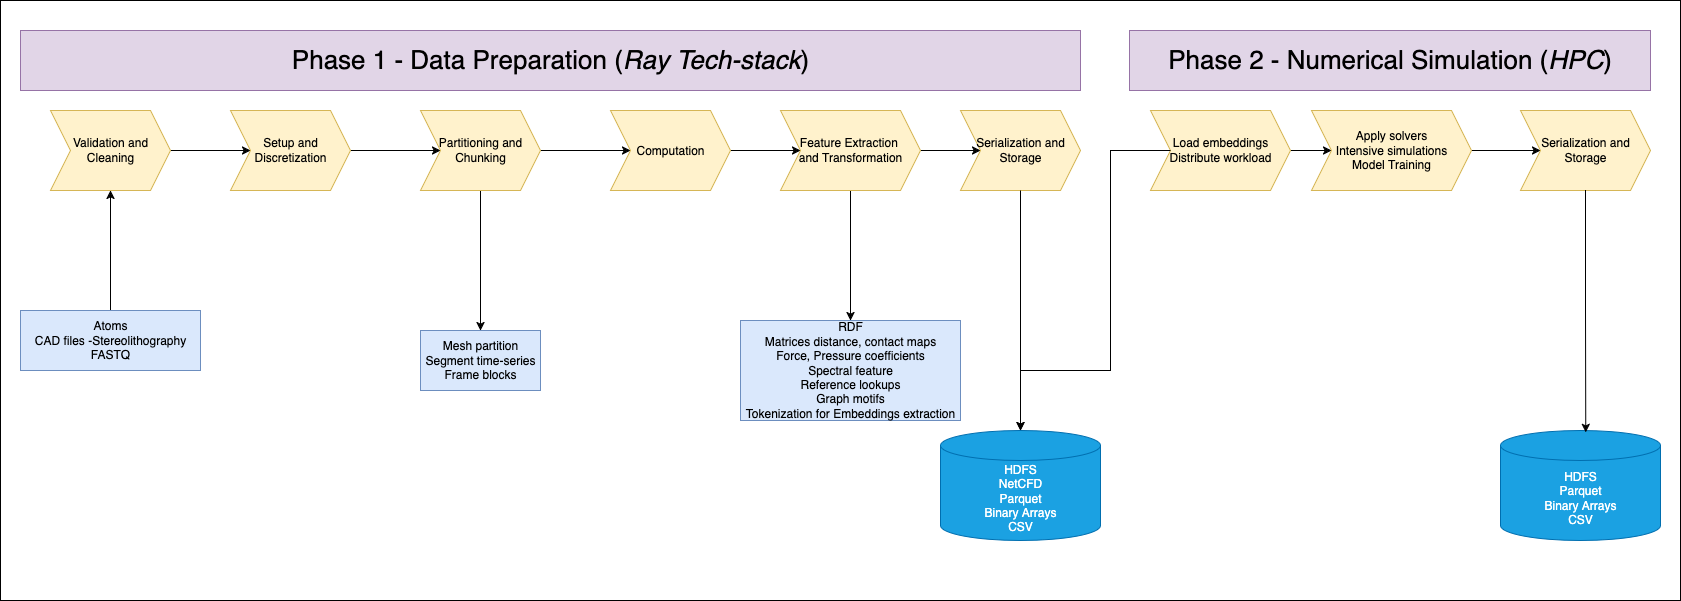
\includegraphics[width=0.9\textwidth,height=0.4\textheight,keepaspectratio]{Generalized_data-pipeline.drawio.png}
    \end{center}
    
    \vspace{0.3cm}
    \begin{block}{Workload Example}
        \textbf{Metagenomics pipeline}  - FASTQ reads → k-mer embeddings → organism clustering
    \end{block}
\end{frame}




% Slide 4: Two-Phased Architecture
\begin{frame}{A Two-Phased Cloud-Native Architecture for Optimization}
    \begin{center}
        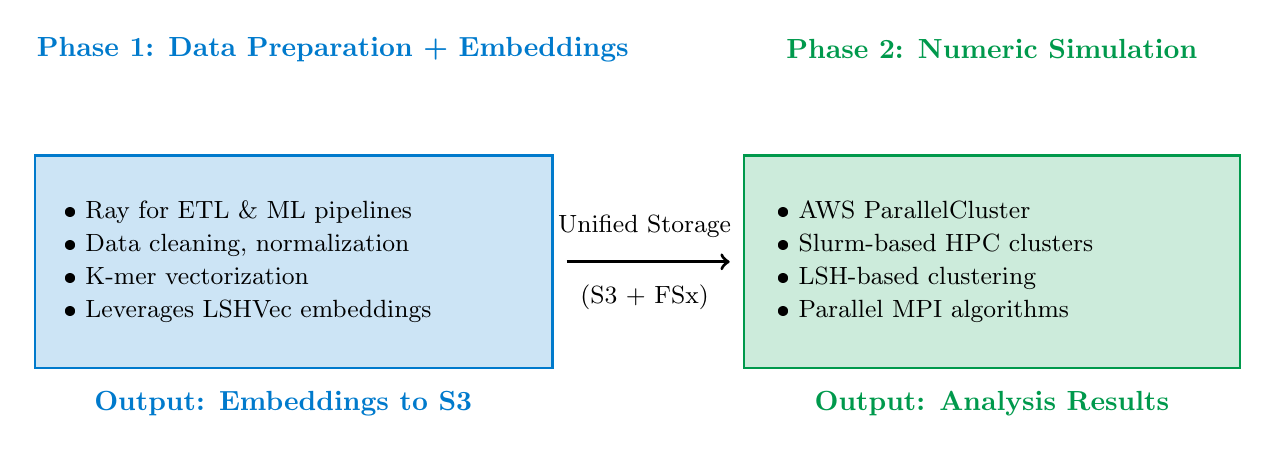
\begin{tikzpicture}[scale=0.9]
            % Phase 1 box
            \draw[thick, rayblue, fill=rayblue!20] (-3,0) rectangle (4.3,3);
            \node[rayblue, font=\bfseries] at (1.2,4.5) {Phase 1: Data Preparation + Embeddings};
            \node[align=left] at (0.0,1.5) {
                \small • Ray for ETL \& ML pipelines \\
                \small • Data cleaning, normalization \\
                \small • K-mer vectorization \\
                \small • Leverages LSHVec embeddings
            };
            \node[rayblue] at (0.5,-0.5) {\textbf{Output: Embeddings to S3}};
            
            % Arrow
            \draw[->, very thick, black] (4.5, 1.5) -- (6.8, 1.5);
            \node at (5.6, 2) {\small Unified Storage};
            \node at (5.6, 1) {\small (S3 + FSx)};
            
            % Phase 2 box
            \draw[thick, hpcgreen, fill=hpcgreen!20] (7,0) rectangle (14,3);
            \node[hpcgreen, font=\bfseries] at (10.5,4.5) {Phase 2: Numeric Simulation};
            \node[align=left] at (9.7,1.5) {
                \small • AWS ParallelCluster \\
                \small • Slurm-based HPC clusters \\
                \small • LSH-based clustering \\
                \small • Parallel MPI algorithms
            };
            \node[hpcgreen] at (10.5,-0.5) {\textbf{Output: Analysis Results}};
        \end{tikzpicture}
    \end{center}
    
    \vspace{0.3cm}
    \begin{block}{Key Integration}
        \textbf{Unified storage layer}: seamless data flow and high-throughput access
    \end{block}
    

\end{frame}

% Slide 3: Phase 1 Deep Dive
\begin{frame}{Phase 1 Deep Dive: Ray for Scalable Data Preprocessing}
    \begin{columns}
        \begin{column}{0.5\textwidth}
            \textbf{Ray's Role in Data Preparation:}
            \begin{itemize}
                \item \textbf{Data Ingestion:} Raw FASTQ reads processing
                \item \textbf{K-mer Embeddings:} Using \textcolor{rayblue}{\textbf{DNABERT-2-117M}} for fixed-length numeric vectors
                \item \textbf{Parallel Processing:} Lightweight tasks across CPUs/GPUs
                \item \textbf{Output:} Parquet shards to Amazon S3
            \end{itemize}
        \end{column}
        \begin{column}{0.5\textwidth}
            \textbf{Performance \& Efficiency:}
            \begin{table}[h]
                \centering
                \small
                \begin{tabular}{lc}
                    \toprule
                    \textbf{Metric} & \textbf{Result} \\
                    \midrule
                    Scaling (1→2 GPUs) & 2× throughput \\
                    Processing rate & ~22 MB/s \\
                    Node startup time & ~90s \\
                    Spot Instance savings & \textcolor{green}{\textbf{65\%}} \\
                    Cost per GB & \textcolor{green}{\textbf{\$0.12}} \\
                    \bottomrule
                \end{tabular}
            \end{table}
        \end{column}
    \end{columns}
    
    \vspace{0.3cm}
    \begin{alertblock}{Key Achievement}
        \textbf{Near-linear scaling} with Ray autoscaler dynamically managing cluster size and achieving \textcolor{green}{\textbf{65\% cost reduction}} through Spot Instances
    \end{alertblock}
\end{frame}

% Slide 4: Phase 2 Deep Dive
\begin{frame}{Phase 2 Deep Dive: HPC for Compute-Intensive Simulation \& Overall Impact}
    \begin{columns}
        \begin{column}{0.6\textwidth}
            \textbf{HPC Simulation with AWS ParallelCluster:}
            \begin{itemize}
                \item \textbf{Embedding Consumption:} Direct access from FSx/S3
                \item \textbf{Specialized Compute:} P4d instances with \textcolor{awsorange}{\textbf{NVIDIA A100 GPUs}}
                \item \textbf{Low-latency Communication:} Elastic Fabric Adapter (EFA) for MPI
                \item \textbf{Clustering Algorithms:} Parallel LSH and k-means for organism grouping
            \end{itemize}
        \end{column}
        \begin{column}{0.4\textwidth}
            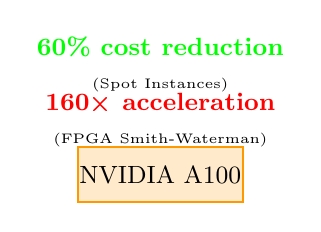
\begin{tikzpicture}[scale=0.7]
                % GPU representation
                \draw[thick, awsorange, fill=awsorange!20] (0,0) rectangle (3,1);
                \node at (1.5,0.5) {\small NVIDIA A100};
                
                % Performance metrics
                \node[align=center] at (1.5,1.5) {\small \textcolor{red}{\textbf{160× acceleration}} \\ \tiny (FPGA Smith-Waterman)};
                
                % Cost savings
                \node[align=center] at (1.5,2.5) {\small \textcolor{green}{\textbf{60\% cost reduction}} \\ \tiny (Spot Instances)};
            \end{tikzpicture}
        \end{column}
    \end{columns}
    
    \vspace{0.3cm}
    \begin{block}{Synergistic Performance \& Benefits}
        \begin{itemize}
            \item \textbf{Hardware Acceleration:} FPGAs achieve \textcolor{red}{\textbf{160-fold acceleration}} for Smith-Waterman algorithms
            \item \textbf{Extreme-scale Processing:} GPU-enabled protein similarity searches across hundreds of millions of proteins in hours vs. weeks
            \item \textbf{Cost Optimization:} \textcolor{green}{\textbf{Over 60\% infrastructure cost reduction}} through Spot Instances
            \item \textbf{Developer Agility:} Unified cloud-agnostic control plane streamlines complex pipelines
        \end{itemize}
    \end{block}
\end{frame}

% Slide 5: Conclusions
\begin{frame}{Conclusions}
    \begin{columns}
        \begin{column}{0.6\textwidth}
            \textbf{Key Conclusions:}
            \begin{itemize}
                \item Two-phase architecture delivers \textbf{significant gains} in scalability, elasticity, performance, and cost-efficiency
                \item \textcolor{rayblue}{\textbf{GPU-accelerated Ray clusters scale nearly linearly}} for DNA embedding extraction
                \item Automated lifecycle management and Spot Instances ensure \textcolor{green}{\textbf{optimized resource utilization}}
                \item Successfully \textbf{decouples feature engineering from raw simulation workloads}
            \end{itemize}
        \end{column}
        \begin{column}{0.4\textwidth}
            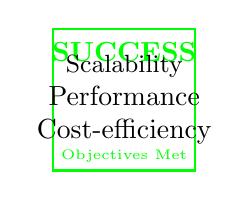
\begin{tikzpicture}[scale=0.6]
                % Success metrics visualization
                \draw[thick, green] (0,0) -- (0,3) -- (3,3) -- (3,0) -- cycle;
                \node[green, font=\bfseries] at (1.5,2.5) {SUCCESS};
                \node[align=center] at (1.5,1.5) {\small Scalability \\ Performance \\ Cost-efficiency};
                \node[green] at (1.5,0.3) {\tiny Objectives Met};
            \end{tikzpicture}
        \end{column}
    \end{columns}
    
    \vspace{0.3cm}
    \begin{block}{Key achievements}
        \begin{itemize}
            \item \textbf{Ray autoscaler - EC2 + GPU:} Explore ... \textcolor{red}{\textbf{orders-of-magnitude speedups}}
            \item \textbf{Storage at scale S3 FsxLustre:} data exchange
            \item \textbf{HPC ParallelCluster and EFA:} Balance ...
        \end{itemize}
    \end{block}
\end{frame}

% Slide 6: Future Directions
\begin{frame}{Future Directions}
    \begin{columns}
        \begin{column}{0.6\textwidth}
            \textbf{Key Emerging Capabilities:}
            \begin{itemize}
                \item Two-phase architecture delivers \textbf{significant gains} in scalability, elasticity, performance, and cost-efficiency
                \item \textcolor{rayblue}{\textbf{GPU-accelerated Ray clusters scale nearly linearly}} for DNA embedding extraction
                \item Automated lifecycle management and Spot Instances ensure...
                \item Successfully \textbf{decouples feature ...}
            \end{itemize}
        \end{column}
        \begin{column}{0.4\textwidth}
            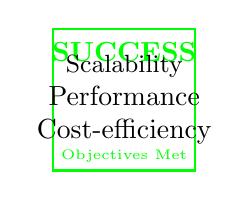
\begin{tikzpicture}[scale=0.6]
                % Success metrics visualization
                \draw[thick, green] (0,0) -- (0,3) -- (3,3) -- (3,0) -- cycle;
                \node[green, font=\bfseries] at (1.5,2.5) {SUCCESS};
                \node[align=center] at (1.5,1.5) {\small Scalability \\ Performance \\ Cost-efficiency};
                \node[green] at (1.5,0.3) {\tiny Objectives Met};
            \end{tikzpicture}
        \end{column}
    \end{columns}
    
    \vspace{0.3cm}
    \begin{block}{Future Work \& Research Avenues}
        \begin{itemize}
            \item \textbf{FPGA Workloads:} Explore AWS F1 instances using Xilinx Vitis for \textcolor{red}{\textbf{orders-of-magnitude speedups}}
            \item \textbf{Apple M-Series SoCs:} Ray's  macOS  edge 
            \item \textbf{Managed ETL \& Conversational DevOps:} agentic AI integrate \textcolor{rayblue}{\textbf{domain-aware LLM agents}} for automated CloudFormation/CDK generation
        \end{itemize}
    \end{block}
\end{frame}

% Slide 2: The New Frontier
\begin{frame}{Studied Topics}
    \begin{center}
        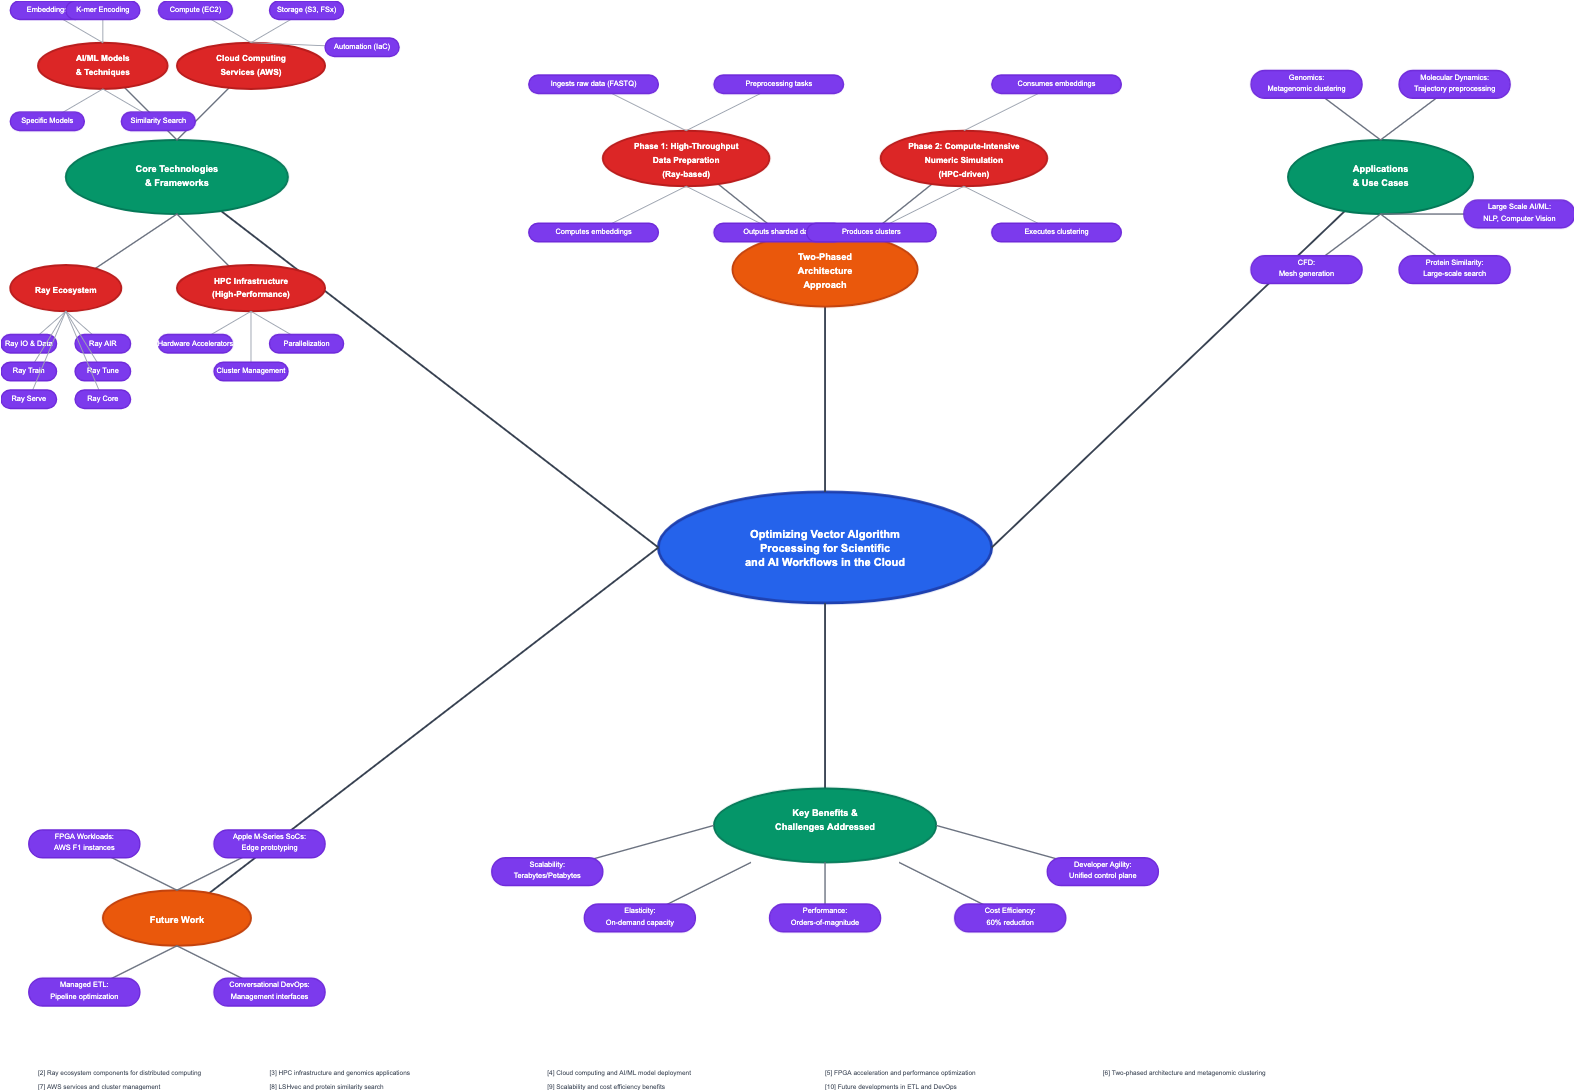
\includegraphics[width=0.9\textwidth,height=0.6\textheight,keepaspectratio]{TFM-MindMap.drawio.png}
    \end{center}
    
    \vspace{0.3cm}
    \begin{block}{Centric idea}
        \textbf{Unified storage layer} bridges Phase 1 outputs with Phase 2 inputs, enabling seamless data flow and high-throughput access
    \end{block}
\end{frame}

% Thank you slide
\begin{frame}[plain]
    \begin{center}
        \Huge Thank You!
        
        \vspace{1cm}
        \Large Questions?
        
        \vspace{0.8cm}
        \normalsize
        \textbf{Optimizing Vector Algorithm Processing through the integration of Ray IO and HPC in the Cloud}
        
        \vspace{0.5cm}
        Tiago de Souza de Oliveira \\
        \texttt{tiago.souza@rai.usc.es, tiagoooliveira@qmind-lab.com}
    \end{center}
\end{frame}

\end{document}